\section{Durchführung}
\label{sec:Durchführung}
\subsection{Messverfahren mittels Induktivitätsbrücke}
Bei der Messung wird die Tatsache ausgenutzt, dass die Suszeptibilität dort messbar ist wo Magnetfelder in Materie
wirken, daher kann die Suszeptibilität mittels Induktivitätsbrücke, zu sehen in Abbildung \ref{fig:brücke}, gemessen werden.
\begin{figure}
  \centering
  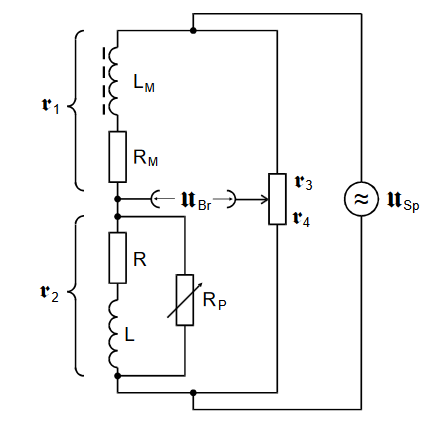
\includegraphics[width=0.4\textwidth]{bruecke.PNG}
  \caption{Induktivitätsbrücke zur Messung der Suszeptibilität. }
  \label{fig:bruecke}
\end{figure}
Diese Brücke besizt zwei Spulen gleicher Induktivität.
Bei der ersten Möglichkeit die Suszeptibilität zu bestimmen, wird die Brücke abgegelichen und anschließend die Probe in eine Spule eingeführt.
Über die entstandene Brückenspannung bestimmt sich die Suszeptibilität folgendermaßen:
\begin{align}
 \Chi(\omega\textrightarrow\infty)=4\frac{FU_\mathrm{Br}}{QU_\mathrm{Sp}}.
\end{align}
Hier bedeutet $F$ der Queerschnitt der Spule und $U_\mathrm{Sp}$ die Speisespannung.

Die zweite Möglichkeit basiert auf der Änderung des Widerstandes $R_3$, dabei wird die abgeglichene Brücke mit der Probe versehen
und erneut abgeglichen. Die Suszeptibilität ergibt sich folgendermaßen:
\begin{align}
\Chi=2\frac{\Delta R F}{R_\mathrm{3} Q}.
\end{align}


\subsection{Voreinstellungen}
Bei dem Messverfahren kommt es zu Störsignalen, die  die Brückenspannung komplett überdecken können, daher ist es sinnvoll
einen Selektivverstärker einzusetzen. Der Selektivverstärker setzt sich zusammen aus der filternden Komponente, diese
lässt im Idealfall die gesuchte, monofrequente Signalspannung durch, und einer verstärkenden Komponente, zur besseren Messung
der Brückenspannung. Zu Beginn wird die filternde Frequenz gesucht, zu diesem Zweck wird ein Spannungsgenerator an den Selektivverstärker
angeschlossen. Nun lässt sich die Frequenz variieren und die zugehörige Spannung kann am Voltmeter abgelesen werden.
Gemessen wird zwischen $30.000-40.000 \si{herz}$ in sinnvollen Schritten, d.h. im Bereich des Maximums wird in kleinschrittiger gemessen
als außerhalb. Die Abbildung \ref{fig:sv} zeigt den Aufbau der genutzten Komponenten.
\begin{figure}
  \centering
  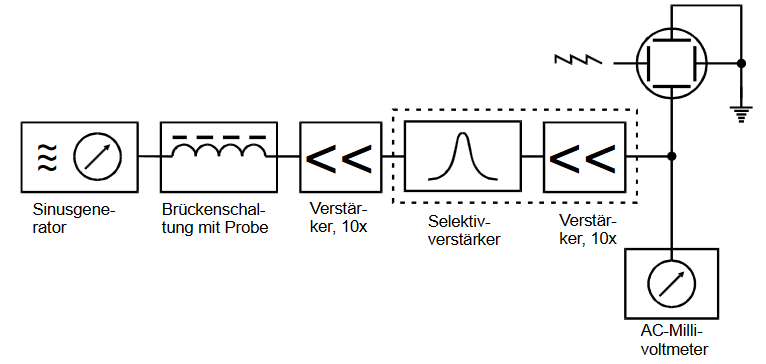
\includegraphics[width=0.6\textwidth]{Selektiv.PNG}
  \caption{Aufbau der verwendeten Apparatur.}
  \label{fig:sv}
\end{figure}


\subsection{Eigentliche Messung}
Bei der eigentlichen Messung wurde zu Beginn die Länge der Probe vermessen.
Am Generator wurde eine Speisespannung von $1\si{\volt}$ eingestellt.
Nach dem Abgleichen der Brücke wurde der Widerstand gemessen und die Probe eingeschoben, dann wird die Brückenspannung $U_\mathrm{Br}$
gemessen und die Brücke abgeglichen, zuletzt wird erneut der Widerstand aufgenommen. Diese Abfolge wird pro Probe drei mal wiederholt.
